% factorizacion_qr

\subsection{Matrices Ortogonales}\label{subsec:matrices_ortogonales}

$Q \in \mathbb{R}^{n \times n}$, $Q$ es ortogonal sí y solo sí $QQ^t = Q^t Q = I$.

\begin{itemize}
    \item[-] Columnas ortogonales denorma $2$ igual a $1$.
    \item[-] Filas ortogonales de norma $2$ igual a $1$.
    \item[-] ${||Q||}_{2} = 1$.
    \item[-] $\kappa_{2}(Q) = 1$.
    \item[-] ${||Qx||}_{2} = {||x||}_{2}$
    \item[-] Producto de ortogonales es ortogonal.
\end{itemize}

\subsection{Factorización QR}\label{subsec:proposicion_fact_qr}

Sean $A \in \mathbb{R}^{n \times n}$, $Q \in \mathbb{R}^{n \times n}$ matriz ortogonal y $R \in \mathbb{R}^{n \times n}$ traingular superior tal que

\[A = QR\]

\noindent De forma que

\[Ax = b\]
\[QRx = b\]
\[Q^{t}QRx = Q^{t}b\]
\[Rx = Q^{t}b\]

Sistema triangular superior, $O(n^2)$.

\subsection{Método de Givens (rotaciones)}\label{subsec:metodo_de_givens}

Dado un ángulo $\theta$, sea la transformación lineal que rota a todo vector del plano en el ángulo $\theta$ en sentido horario.

\

\begin{multicols}{2}
    
    \begin{center}    
        \begin{tikzpicture}
            \draw [-to] (0,-1) -- (0,2);
            \draw [-to] (-1,0) -- (2,0);
            \draw [-to,blue] (0,0) -- (1,2);
            \draw [-to,blue,dashed] (0,0) -- (2,1);
            \draw [-to,blue] (0.6,1) arc (60:30:1);
            \node [blue] at (1,1) {\small $\theta$};
            \node at (2.2,0) {$x$};
            \node at (0,2.2) {$y$};
        \end{tikzpicture}
    \end{center}    
    
    \
    
    $W = 
    \begin{bmatrix}
        cos(\theta) & sen(\theta) \\
        -sen(\theta) & cos(\theta)
    \end{bmatrix}
    $

    \

    \

    $W$ es ortonogal y ${||Wx||}_{2} = {||x||}_{2}$

\end{multicols}

Dados $\tilde{x},\tilde{y} \in \mathbb{R}^{2},\tilde{y} = \begin{bmatrix}
    {||\tilde{x}||}_{2} \\
    0
\end{bmatrix}$, se busca la rotación $W$ tal que $W\tilde{x} = \tilde{y}$

\

\begin{multicols}{2}    
    
    \begin{center}
        \begin{tikzpicture}
            \draw [-to] (0,-1) -- (0,2);
            \draw [-to] (-1,0) -- (0,0);
            \draw [-to] (1.5,0) -- (2,0);
            \draw [-to,blue] (0,0) -- (1,1.5);
            \draw [-to,blue,dashed] (0,0) -- (1.5,0);
            \draw [-to,blue] (0.7,0.9) arc (60:0:1);
            \node [blue] at (1.2,0.8) {\small $?$};
            \node at (2.2,0) {$x$};
            \node [blue] at (1.1,1.7) {$\tilde{x}$};
            \node at (0,2.2) {$y$};
            \node [blue] at (1.6,-0.2) {$\tilde{y}$};
        \end{tikzpicture}
    \end{center}
    
    \

    \

    \scalebox{1.3}{$W = 
    \begin{bmatrix}
        \frac{\tilde{x}_1}{{||\tilde{x}||}_2} & \frac{\tilde{x}_2}{{||\tilde{x}||}_2} \\
        -\frac{\tilde{x}_2}{{||\tilde{x}||}_2} & \frac{\tilde{x}_1}{{||\tilde{x}||}_2}
    \end{bmatrix}
    $}

\end{multicols}

Sean $A \in \mathbb{R}^{n \times n}, \tilde{x} = \begin{bmatrix}
    a_{11} \\ a_{21}
\end{bmatrix}$ y $\tilde{y} = \begin{bmatrix}
    {||\tilde{x}||}_{2} \\ 0
\end{bmatrix}$.


Existe $W \in \mathbb{R}^{2 \times 2}$ tal que $W\tilde{x} = \tilde{y}$. Sea

\[
W_{12} =
\begin{bmatrix}
    w_{11} & w_{12} & 0 & \ldots & 0 \\
    w_{21} & w_{22} & 0 & \ldots & 0 \\
    0 & 0 & 1 & \ldots & 0 \\
    \vdots & \vdots & \vdots & \ddots & \vdots \\
    0 & 0 & 0 & \ldots & 1 \\
\end{bmatrix}
\]

donde si se realiza el siguiente producto

\[
W_{12}A =
\begin{bmatrix}
    * & * & \ldots & * \\
    \textcolor{red}{0} & * & \ldots & * \\
    a_{31} & a_{32} & \ldots & a_{3n} \\
    \vdots & \vdots & \ddots & \vdots \\
    a_{n1} & a_{n2} & \ldots & a_{nn} \\
\end{bmatrix}
=
\begin{bmatrix}
    a_{11}^{1} & a_{12}^{1} & \ldots & a_{1n}^{1} \\
    \textcolor{red}{0} & a_{22}^{1} & \ldots & a_{2n}^{1} \\
    a_{31}^{1} & a_{32}^{1} & \ldots & a_{3n}^{1} \\
    \vdots & \vdots & \ddots & \vdots \\
    a_{n1}^{1} & a_{n2}^{1} & \ldots & a_{nn}^{1} \\
\end{bmatrix}
\]

\

\noindent De esta forma se puede contiguar con el siguiente paso, sean $\tilde{x} = \begin{bmatrix}
    a_{11}^1 \\ a_{31}^1
\end{bmatrix}$ y $\tilde{y} = \begin{bmatrix}
    {||\tilde{x}||}_{2} \\ 0
\end{bmatrix}$.

Existe $W \in \mathbb{R}^{2 \times 2}$ tal que $W\tilde{x} = \tilde{y}$. Sea

\[
W_{13} =
\begin{bmatrix}
    w_{11} & 0 & w_{13} & \ldots & 0 \\
    0 & 1 & 0 & \ldots & 0 \\
    w_{31} & 0 & w_{33} & \ldots & 0 \\
    \vdots & \vdots & \vdots & \ddots & \vdots \\
    0 & 0 & 0 & \ldots & 1 \\
\end{bmatrix}
\]

donde si se realiza el siguiente producto

\[
W_{13}W_{12}A =
\begin{bmatrix}
    * & * & \ldots & * \\
    \textcolor{red}{0} & * & \ldots & * \\
    \textcolor{red}{0} & * & \ldots & * \\
    \vdots & \vdots & \ddots & \vdots \\
    a_{n1} & a_{n2} & \ldots & a_{nn} \\
\end{bmatrix}
=
\begin{bmatrix}
    a_{11}^{2} & a_{12}^{2} & \ldots & a_{1n}^{2} \\
    \textcolor{red}{0} & a_{22}^{2} & \ldots & a_{2n}^{2} \\
    \textcolor{red}{0} & a_{32}^{2} & \ldots & a_{3n}^{2} \\
    \vdots & \vdots & \ddots & \vdots \\
    a_{n1}^{2} & a_{n2}^{2} & \ldots & a_{nn}^{2} \\
\end{bmatrix}
\]


De forma similar, para la posición $i1$ , sean $\tilde{x} = \begin{bmatrix}
    a_{11}^{i-1} \\ a_{i1}^1
\end{bmatrix}$ y $\tilde{y} = \begin{bmatrix}
    {||\tilde{x}||}_{2} \\ 0
\end{bmatrix}$.

Existe $W \in \mathbb{R}^{2 \times 2}$ tal que $W\tilde{x} = \tilde{y}$. Sea

\[
W_{1i} =
\begin{bmatrix}
    w_{11} & 0 & \ldots & w_{1i} & 0 & \ldots & 0 \\
    0 & 1 & \ldots & 0 & 0 & \ldots & 0 \\
    \vdots & \vdots & \ddots & \vdots & \vdots & \ddots & \vdots \\
    w_{i1} & 0 & \ldots & w_{ii} & 0 & \ldots & 0 \\
    \vdots & \vdots & \ddots & \vdots & \vdots & \ddots & \vdots \\
    0 & 0 & \ldots & 0 & 0 & \ldots & 1 \\
\end{bmatrix}
\]

\

donde si se realiza el siguiente producto con $i = n$

\[
W_{1n}\cdots W_{13}W_{12}A =
\begin{bmatrix}
    * & * & \ldots & * \\
    \textcolor{red}{0} & * & \ldots & * \\
    \textcolor{red}{0} & * & \ldots & * \\
    \textcolor{red}{\vdots} & \vdots & \ddots & \vdots \\
    \textcolor{red}{0} & * & \ldots & * \\
\end{bmatrix}
=
\begin{bmatrix}
    a_{11}^{(n-1)} & a_{12}^{(n-1)} & \ldots & a_{1n}^{(n-1)} \\
    \textcolor{red}{0} & a_{22}^{(n-1)} & \ldots & a_{2n}^{(n-1)} \\
    \textcolor{red}{0} & a_{32}^{(n-1)} & \ldots & a_{3n}^{(n-1)} \\
    \textcolor{red}{\vdots} & \vdots & \ddots & \vdots \\
    \textcolor{red}{0} & a_{n2}^{(n-1)} & \ldots & a_{nn}^{(n-1)} \\
\end{bmatrix}
\]

\subsubsection{Esquema}\label{subsubsec:givens_esquema}

Para $i = 1,\ldots,n-1$, $j = i+1,\ldots,n$, sea

\[
W_{ij} =
\begin{bmatrix}    
    1 & \ldots & 0 & \ldots & 0 & \ldots & 0 \\
    \vdots & \ddots & \vdots & \ddots & \vdots & \ddots & \vdots \\
    0 & \ldots & w_{ii} & \ldots & w_{ij} & \ldots & 0 \\
    \vdots & \ddots & \vdots & \ddots & \vdots & \ddots & \vdots \\
    0 & \ldots & w_{ji} & \ldots & w_{jj} & \ldots & 0 \\
    \vdots & \ddots & \vdots & \ddots & \vdots & \ddots & \vdots \\
    0 & \ldots & 0 & \ldots & 0 & \ldots & 1 \\
\end{bmatrix}
\]

\

luego, con estas matrices tengo el siguiente producto

\[W_{n-1n}W_{n-2n}W_{n-1n-1}\cdots W_{1n}\cdots W_{12}A = R\]
\[A = W_{12}^{t}\cdots W_{1n}^{t}\cdots W_{n-2n-1}^{t}W_{n-2n}^{t}W_{n-1n}R\]
\[A = QR\]

\subsubsection{Costo}\label{subsubsec:givens_costo}

\[W_{n-1n}W_{n-2n}W_{n-1n-1}\cdots W_{1n}\cdots W_{12}A = R\]

\

\noindent Calcular cada $W_{ij}$: $2$ productos + $2$ cocientes + $1$ raiz.

\begin{itemize}
    \item[-] Primera Columna:
             $W_{1j}$ actúa entre las filas $1$ y $j$ para $j = 2,\ldots,n$

             Costo: $4n$ productos + $2n$ sumas
              
             Costo total: $(n-1)(4n + 2n + 2 + 2 + 1)$
    \item[-] i-ésima Columna:
             $W_{ij}$ actúa entre las filas $i$ y $j$ para $j = i+1,\ldots,n$

             Costo: $4(n-i+1)$ productos + $2(n -i +1)$ sumas

             Costo total: $(n-1)(4(n - i + 1) + 2(n - i + 1) + 2 + 2 + 1)$
\end{itemize}

\noindent Costo total del algoritmo:

\[\sum_{i=1}^{n-1}(n-i)(4(n - i + 1) + 2(n - i + 1) + 2 + 2 + 1) ~\in O(\frac{4}{3}n^3)\]

\newpage

\subsubsection{Ejemplo}\label{subsubsec:givens_ejemplo}

Se tiene

\[
A = 
\begin{bmatrix}
     0 & -20 & -14 \\
     3 & 27 & -4 \\
     4 & 1 & -2
\end{bmatrix}
\]

\

y sea $\tilde{x} = (3,0)$, buscamos $W$, rotación en plano, tal que $W\tilde{x} = \tilde{y}$ con $\tilde{y} = (0,3)$.

\

\begin{center}    
\scalebox{1.3}{
$
W = 
\begin{bmatrix}
    \frac{\tilde{x}_1}{{||\tilde{x}||}_{2}} & \frac{\tilde{x}_2}{{||\tilde{x}||}_{2}} \\
    -\frac{\tilde{x}_2}{{||\tilde{x}||}_{2}} & \frac{\tilde{x}_1}{{||\tilde{x}||}_{2}} \\
\end{bmatrix}
= 
\begin{bmatrix}
    \frac{0}{3} & \frac{3}{3} \\
    -\frac{3}{3} & \frac{0}{3}
\end{bmatrix}
\implies
W_{12} = 
\begin{bmatrix}
    0 & 1 & 0 \\
    -1 & 0 & 0 \\
    0 & 0 & 1
\end{bmatrix}
$
}
\end{center}

luego con esta información se procede a calcular $W_{12}A$, de forma que

\[
W_{12}A = 
\begin{bmatrix}
    0 & 1 & 0 \\
    -1 & 0 & 0 \\
    0 & 0 & 1
\end{bmatrix}
\begin{bmatrix}
    0 & -20 & -14 \\
    3 & 27 & -4 \\
    4 & 1 & -2
\end{bmatrix}
=
\begin{bmatrix}
    3 & 27 & -4 \\
    \textcolor{red}{0} & 20 & 14 \\
    4 & 11 & -2
\end{bmatrix}
\]

\

Sea $\tilde{x} = (3,4)$, buscamos $W$, rotación en el plano tal que $W\tilde{x} = \tilde{y}$ con $\tilde{y} = (5,0)$

\begin{center}    
\scalebox{1.3}{
$
W = 
\begin{bmatrix}
    \frac{\tilde{x}_1}{{||\tilde{x}||}_{2}} & \frac{\tilde{x}_2}{{||\tilde{x}||}_{2}} \\
    -\frac{\tilde{x}_2}{{||\tilde{x}||}_{2}} & \frac{\tilde{x}_1}{{||\tilde{x}||}_{2}} \\
\end{bmatrix}
= 
\begin{bmatrix}
    \frac{3}{5} & \frac{4}{5} \\
    -\frac{4}{5} & \frac{3}{5}
\end{bmatrix}
\implies
W_{13} = 
\begin{bmatrix}
    \frac{3}{5} & 0 & \frac{4}{5} \\
    0 & 1 & 0 \\
    -\frac{4}{5} & 0 & \frac{3}{5}
\end{bmatrix}
$
}
\end{center}

y con esta información se procede a calcular $W_{13}W_{12}A$, de forma que

\[
W_{13}W_{12}A = 
\begin{bmatrix}
    \frac{3}{5} & 0 & \frac{4}{5} \\
    0 & 1 & 0 \\
    -\frac{4}{5} & 0 & \frac{3}{5}
\end{bmatrix}
\begin{bmatrix}
    3 & 27 & -4 \\
    \textcolor{red}{0} & 20 & 14 \\
    4 & 11 & -2
\end{bmatrix}
=
\begin{bmatrix}
    5 & 25 & -4 \\
    \textcolor{red}{0} & 20 & 14 \\
    \textcolor{red}{0} & 13 & -2
\end{bmatrix}
\]

\

por último, sea $\tilde{x} = (20,-15)$, buscamos $W$, rotación en el plano tal que $W\tilde{x} = \tilde{y}$ con $\tilde{y} = (25,0)$.

\begin{center}    
\scalebox{1.3}{
$
W = 
\begin{bmatrix}
    \frac{\tilde{x}_1}{{||\tilde{x}||}_{2}} & \frac{\tilde{x}_2}{{||\tilde{x}||}_{2}} \\
    -\frac{\tilde{x}_2}{{||\tilde{x}||}_{2}} & \frac{\tilde{x}_1}{{||\tilde{x}||}_{2}} \\
\end{bmatrix}
= 
\begin{bmatrix}
    \frac{20}{25} & -\frac{15}{25} \\
    \frac{15}{25} & \frac{20}{25}
\end{bmatrix}
\implies
W_{23} = 
\begin{bmatrix}
    1 & 0 & 0 \\
    0 & \frac{20}{25} & -\frac{15}{25} \\
    0 & \frac{15}{25} & \frac{20}{25}
\end{bmatrix}
$
}
\end{center}

y se puede realizar el último producto

\[
W_{23}W_{13}W_{12}A = 
\begin{bmatrix}
    1 & 0 & 0 \\
    0 & \frac{20}{25} & -\frac{15}{25} \\
    0 & \frac{15}{25} & \frac{20}{25}
\end{bmatrix}
\begin{bmatrix}
    5 & 25 & -4 \\
    \textcolor{red}{0} & 20 & 14 \\
    \textcolor{red}{0} & 13 & -2
\end{bmatrix}
=
\begin{bmatrix}
    5 & 25 & -4 \\
    \textcolor{red}{0} & 25 & 10 \\
    \textcolor{red}{0} & \textcolor{red}{0} & 10
\end{bmatrix}
\]

Luego, tengo que $A = QR$ con 

\begin{center}    
\scalebox{1.3}{$
Q = W_{12}^{t}W_{13}^{t}W_{23}^{t} = 
\begin{bmatrix}
    0 & -\frac{20}{25} & -\frac{15}{25} \\
    \frac{15}{25} & \frac{12}{25} & -\frac{16}{25} \\
    \frac{20}{25} & -\frac{9}{25} & \frac{12}{25}
\end{bmatrix}
~~~~~~~~~~~
R =
\begin{bmatrix}
    5 & 25 & -4 \\
    \textcolor{red}{0} & 25 & 10 \\
    \textcolor{red}{0} & \textcolor{red}{0} & 10
\end{bmatrix}
$
}
\end{center}

\newpage

\subsection{Método de Householder (reflexiones)}\label{subsec:metodo_de_householder}

\begin{multicols}{2}

    \begin{center}    
        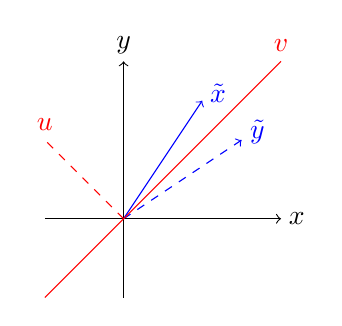
\begin{tikzpicture}
            \draw [-to] (0,-1) -- (0,2);
            \draw [-to] (-1,0) -- (2,0);
            \draw [-to,blue] (0,0) -- (1,1.5);
            \draw [-to,blue,dashed] (0,0) -- (1.5,1);
            \draw [red,dashed] (0,0) -- (-1,1);
            \draw [red] (-1,-1) -- (2,2);
            \node [blue] at (1.2,1.6) {$\tilde{x}$};
            \node [blue] at (1.7,1.1) {$\tilde{y}$};
            \node at (2.2,0) {$x$};
            \node at (0,2.2) {$y$};
            \node [red] at (-1,1.2) {$u$};
            \node [red] at (2,2.2) {$v$};
        \end{tikzpicture}
    \end{center} 
    

    \[H\tilde{x} = \tilde{y}~~~~~~\]

    \[Hu = -u~~~~~~\]

    \[Hv = v~~~~~~\]

\end{multicols}

\

Como $v$ y $u$ forman una base, entonces $\tilde{x} = \alpha v + \beta u$. Además, la reflexión de $\tilde{x}$ es $\tilde{y} = \alpha v - \beta u$.

Entonces, buscamos $H$ tal que $H\tilde{x} = \alpha v - \beta u$
\[\alpha v - \beta u = \alpha v + \beta u - 2\beta u\]
\[H\tilde{x} = I\tilde{x} - W\tilde{x} ~~\text{tal que}~~ W\tilde{x} = \alpha Wv + \beta Wu = 2\beta u\]

y se necesita que $Wv = 0$ y $Wu = 2u$.

\

\noindent Sea $P = uu^t$ y asumamos ${||u||}_{2} = 1$, tenemos que

\begin{itemize}
    \item[-] $P$ es simétrica.
    \item[-] $PP^t = P$.
    \item[-] $Pu = u$.
    \item[-] $Pv = 0$.
\end{itemize}

\noindent Si definimos $W = 2P$, se tiene

\[H = I - 2P\]
\[H\tilde{x} = (I-2P)(\alpha v + \beta u) =\]
\[I(\alpha v + \beta u) - 2P(\alpha v + \beta u) =\]
\[\alpha v + \beta u - 2\beta u = \tilde{y}\]



\subsubsection{Propiedades de H}\label{subsubsec:householder_propiedades_h}

\[H = I - 2uu^t\]

\begin{itemize}
    \item[-] $H$ es simétrica.
    \item[-] $H$ es ortogonal.
\end{itemize}

\

\noindent Sean $\tilde{x},~\tilde{y} \in \mathbb{R}^{n},~\tilde{x} \neq \tilde{y},~{||\tilde{x}||}_{2} = {||\tilde{y}||}_{2}$. Existe una transformación de Householder tal que $H\tilde{x} = \tilde{y}$.

\

\begin{multicols}{2}
    \begin{center}    
        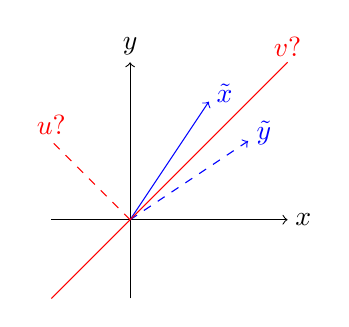
\begin{tikzpicture}
            \draw [-to] (0,-1) -- (0,2);
            \draw [-to] (-1,0) -- (2,0);
            \draw [-to,blue] (0,0) -- (1,1.5);
            \draw [-to,blue,dashed] (0,0) -- (1.5,1);
            \draw [red,dashed] (0,0) -- (-1,1);
            \draw [red] (-1,-1) -- (2,2);
            \node [blue] at (1.2,1.6) {$\tilde{x}$};
            \node [blue] at (1.7,1.1) {$\tilde{y}$};
            \node at (2.2,0) {$x$};
            \node at (0,2.2) {$y$};
            \node [red] at (-1,1.2) {$u?$};
            \node [red] at (2,2.2) {$v?$};
        \end{tikzpicture}
    \end{center} 

    \[v = \tilde{x} + \tilde{y}~~~~~~\]

    \[u = \frac{\tilde{x} - \tilde{y}}{{||\tilde{x}-\tilde{y}||}_{2}}~~~~~~\]

    \[H = I - 2\frac{(\tilde{x}-\tilde{y}){(\tilde{x}-\tilde{y})}^{t}}{{||\tilde{x}-\tilde{y}||}_{2}^{2}}~~~~~~\]
\end{multicols}



\noindent Sean $A \in \mathbb{R}^{2 \times 2},~\tilde{x}=\begin{bmatrix}
    a_{11} \\ a_{21}
\end{bmatrix}$ y $\tilde{y} = \begin{bmatrix}
    {||\tilde{x}||}_{2} \\ 0
\end{bmatrix}$.

\

\noindent Existe $H$ tal que $H\tilde{x} = \tilde{y}$.

 \[HA = \begin{bmatrix}
    {||\tilde{x}||}_{2} & * \\
    0 & *
 \end{bmatrix}\]
 \[HA = R\]
 \[H^{t}HA = H^{t}R\]
 \[A = QR\]

\subsubsection{Costo}\label{subsubsec:householder_costo}

\subsubsection{Ejemplo}\label{subsubsec:householder_ejemplo}

\subsection{Propiedades}\label{subsec:propiedades_qr}